% Master file for Chapter 4: The Catalogue of Tetramers
\section{Tetrameric Geometry}
\label{sec:tetramers-and-scale-models}

The vast majority of composition mosaics on $\mathbb{Z}_{16}$ (specifically, $82{,}884$ of the $83{,}488$ dihedral orbits, or $99.28\%$) gather into closed harmonic four-cycles under the Galois multiplier $\mu_3 \colon x \mapsto 3x \pmod{16}$. Theorem~\ref{thm:spectral-decomposition-z44} establishes that exactly $20{,}721$ such affine tetramers exist.

Within each tetramer cartouche, a complete orbit unfolds in a closed four-cycle:
\begin{equation}
\label{eqn:tetramer-progression}
\mu_1(O) \quad\longrightarrow\quad \mu_3(O) \quad\longrightarrow\quad \mu_7(O) \quad\longrightarrow\quad \mu_5(O) \quad\longrightarrow\quad \mu_1(O)
\end{equation}
Every step corresponds to multiplication by $3 \pmod{16}$, closing after four iterations because $3^4 \equiv 81 \equiv 1 \pmod{16}$.

\subsection{Horizontal Cartouche Geometry}

To make the algebraic sequence immediately and unambiguously readable, each tetramer unfolds in a horizontal linear cartouche ($1 \times 4$ strip). The four mosaics progress naturally from left to right across the page:
\begin{center}
\small
\begin{tabular}{cccc}
\toprule
\textbf{Position 1} & \textbf{Position 2} & \textbf{Position 3} & \textbf{Position 4} \\
\midrule
Root Orbit & First Dilation & Second Dilation (Involution) & Third Dilation (Inverse) \\
$\mu_1 \colon x \mapsto x$ & $\mu_3 \colon x \mapsto 3x$ & $\mu_7 \colon x \mapsto 7x$ & $\mu_5 \colon x \mapsto 5x$ \\
\bottomrule
\end{tabular}
\end{center}
Reading from left to right traces the exact dilation sequence:
\[
\mu_1(O) \;\xrightarrow{\mu_3}\; \mu_3(O) \;\xrightarrow{\mu_3}\; \mu_7(O) \;\xrightarrow{\mu_3}\; \mu_5(O) \;\xrightarrow{\mu_3}\; \mu_1(O)
\]
This linear orientation completely eliminates the ambiguity of two-dimensional grid layouts (where reading order conflicts with cyclic flow), making the location of the canonical root mosaic ($\mu_1$) and each subsequent modular dilation immediately discernible to the eye.

Following the standard clock-face geometry (with vertex $0$ at 12~o'clock and indices advancing clockwise), each inscribed quadrilateral is strictly convex, with its vertices circularly ordered ($v_1 < v_2 < v_3 < v_4$) to avoid self-intersecting chords, and coloured according to the two-colour symmetry taxonomy:
\begin{itemize}
    \item \textbf{Symmetric Blocks (shaded blue)}: Polygons invariant under reflection on $\mathbb{Z}_{16}$, including regular squares $(4,4,4,4)$, rectangles $(1,7,1,7)$, and symmetric trapezoids.
    \item \textbf{Chiral Blocks (shaded pink)}: Polygons lacking reflectional symmetry on $\mathbb{Z}_{16}$, occurring in enantiomorphic pairs.
\end{itemize}

\subsection{Natural Geometric Sorting}

To give the entire universe of $20{,}721$ tetramers a mathematically natural and visually striking progression, every cartouche is indexed according to a 5-tier hierarchical cascade:
\begin{enumerate}
    \item \textbf{Tier 1: Dihedral Orbit Size $|O|$}:
    Arranged in ascending order of dihedral orbit size:
    \[
    |O| \in \{4, 8, 16, 32\}
    \]
    The highest-symmetry orbits ($|O| = 4$ and $|O| = 8$) appear at the very head of the catalogue. Among all $20{,}721$ tetramers, exactly $2$ have orbit size $4$, $21$ have orbit size $8$, $622$ have orbit size $16$, and the remaining $20{,}076$ have orbit size $32$.
    
    \item \textbf{Tier 2: Symmetric Block Count $s$}:
    Within each orbit size, tetramers are sorted by the number of symmetric (achiral) blocks $s \in \{4, 3, 2, 1, 0\}$ in descending order ($4 \to 0$). This induces an unmistakable visual transition: pages begin in pure cobalt blue ($s = 4$), with pink chiral blocks appearing gradually until the final sections display completely chiral patterns ($s = 0$).
    
    \item \textbf{Tier 3: Chord Dispersion Energy $\mathcal{E}(P)$}:
    Sorted in descending order of circular chord dispersion energy:
    \[
    \mathcal{E}(P) = \sum_{B \in P} \sum_{x < y \in B} \min((y - x) \bmod 16, (x - y) \bmod 16)^2
    \]
    High energy corresponds to maximally regular, dispersed polygons with long chords; low energy corresponds to tightly clustered chords.
    
    \item \textbf{Tier 4: Canonical Stride Profile Multiset}:
    Grouping together tetramers whose inscribed quadrilaterals have identical unoriented cyclic stride profiles.
    
    \item \textbf{Tier 5: Canonical Lexicographic Tie-Breaker}:
    Canonical sorted block-set representation on $\mathbb{Z}_{16}$.
\end{enumerate}

The complete machine-readable index of all affine macro-orbits, formatted in this compact single-character notation with full cycle relabelings and chirality signatures, is preserved in the companion resource file \texttt{hexadecality\_index.txt}.

\section{The Complete Catalogue of 20721 Tetramers}
\label{sec:tetramers-catalogue}

Following the 5-tier natural sorting cascade, the complete atlas of all $20{,}721$ affine tetramers on $\mathbb{Z}_{16}$ unfolds across the following 216 plates (96 horizontal linear cartouches per page). Each cartouche presents the canonical orbit sequence $\mu_1 \to \mu_3 \to \mu_7 \to \mu_5$ from left to right. Top-left badges give the sequential tetramer index ($T_1 \dots T_{20721}$); bottom-right numerals state the shared dihedral orbit size $|O| \in \{4, 8, 16, 32\}$. The plate sequence opens with the maximal-symmetry cobalt blue configurations ($s = 4$), transitioning gracefully across descending symmetry tiers to the fully chiral pink compositions ($s = 0$).

\clearpage
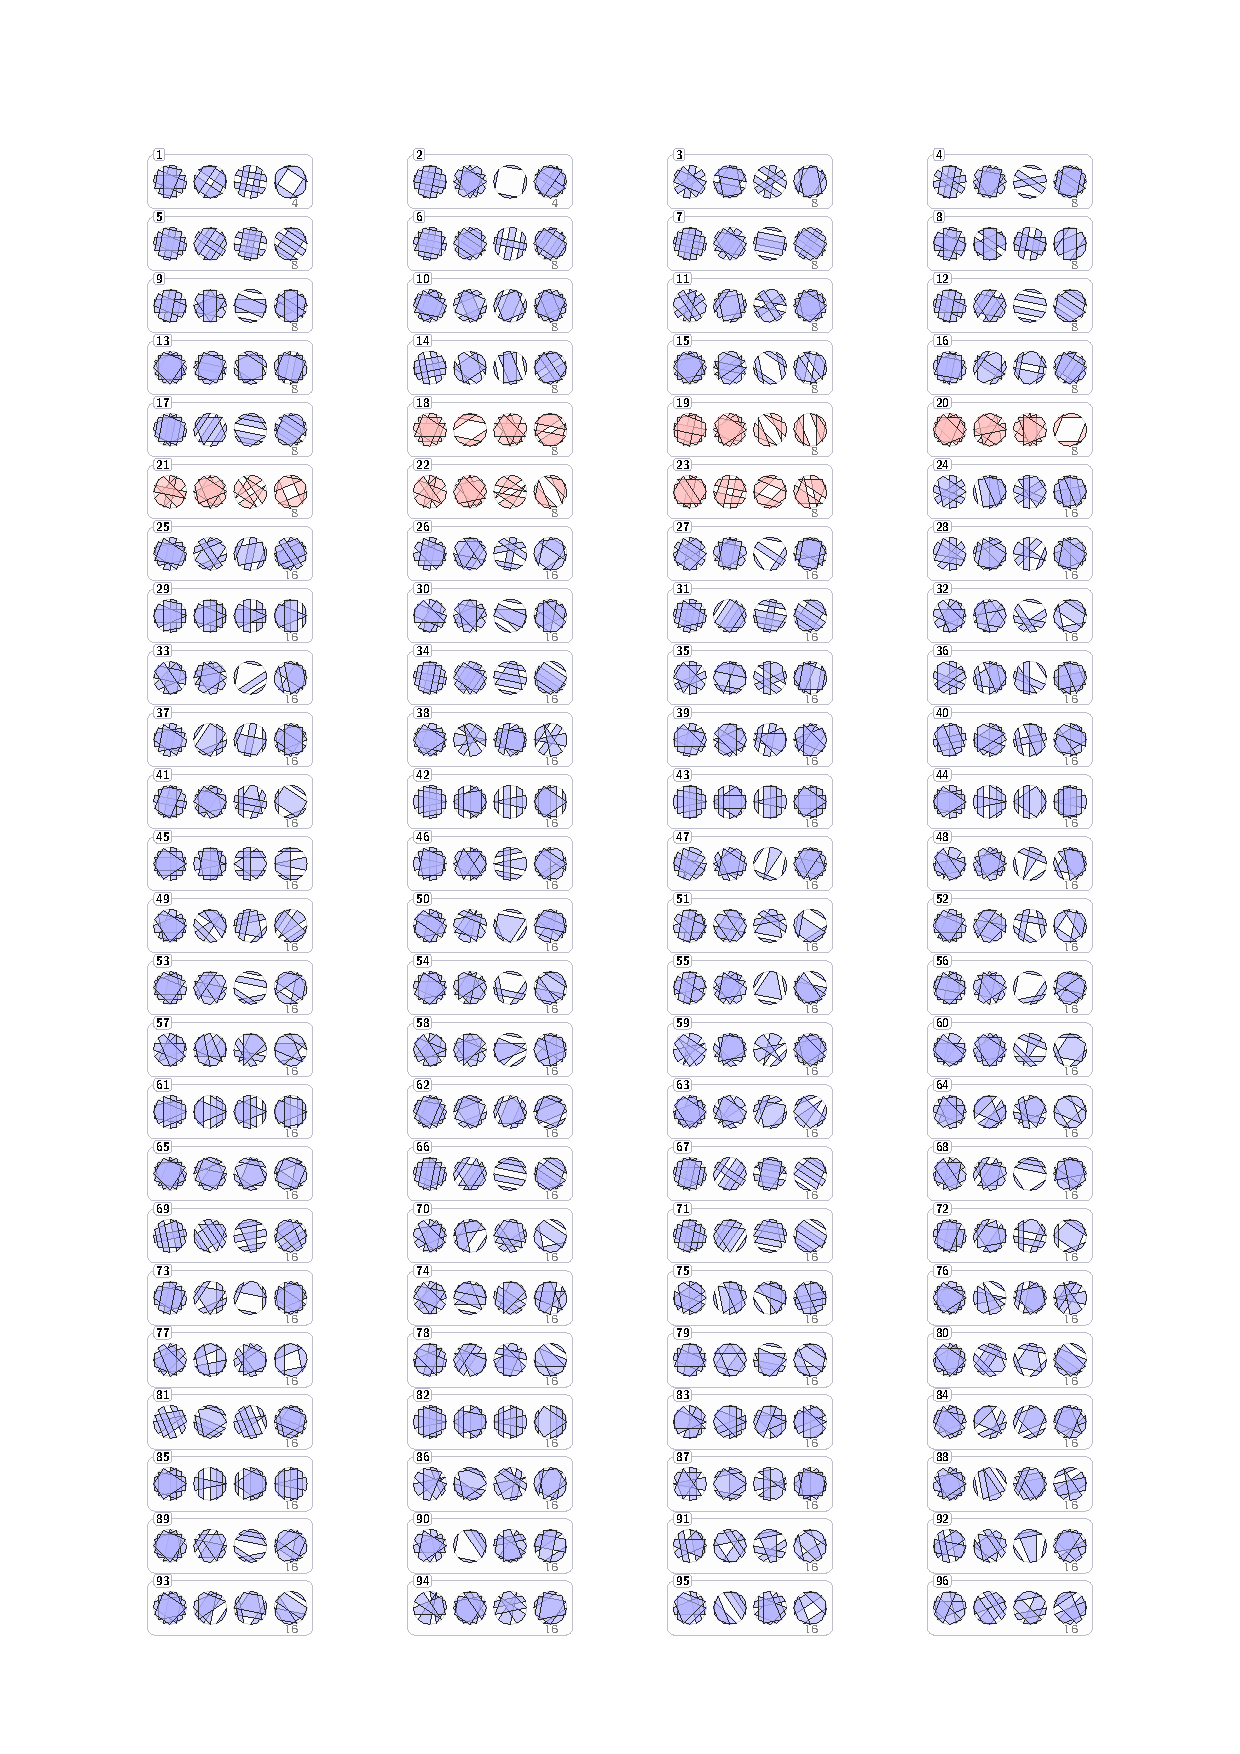
\includepdf[pages=-, pagecommand={\thispagestyle{headings}}]{plates/tetramers_atlas.pdf}
